\documentclass[tikz]{standalone}
\usepackage{tikz}
\usetikzlibrary{positioning, graphs}
\usetikzlibrary{graphs.standard}
\begin{document}
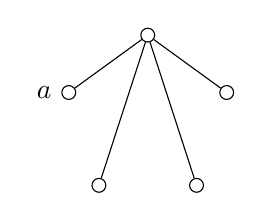
\begin{tikzpicture}
    [mynode/.style={draw,circle,inner sep = 0em, minimum size = 5}]
    \graph[nodes={mynode, empty nodes}, clockwise, radius=30, n=5] {subgraph I_n};

    \node[anchor=east] at (5.west) {$a$};

    \draw (5) -- (1);
    \draw (1) -- (2);
    \draw (1) -- (3);
    \draw (1) -- (4);
\end{tikzpicture}
\end{document}